\documentclass{eecslides}
\usepackage{amsmath}
\usepackage{color}
\usepackage{listings}
\definecolor{lgray}{gray}{0.9}
\lstset{ %
language=R,                		% choose the language of the code
basicstyle=\tiny,       % the size of the fonts that are used for the code
numbers=left,                  	% where to put the line-numbers
numberstyle=\footnotesize,   % the size of the fonts that are used for the line-numbers
stepnumber=1,                   	% the step between two line-numbers. If it is 1 each line will be numbered
numbersep=5pt,                  	% how far the line-numbers are from the code
backgroundcolor=\color{lgray},  % choose the background color. You must add \usepackage{color}
showspaces=false,              	% show spaces adding particular underscores
showstringspaces=false,         % underline spaces within strings
showtabs=false,                 	% show tabs within strings adding particular underscores
frame=single,           		% adds a frame around the code
tabsize=2,          			% sets default tabsize to 2 spaces
captionpos=b,           		% sets the caption-position to bottom
breaklines=true,        		% sets automatic line breaking
breakatwhitespace=false,    	% sets if automatic breaks should only happen at whitespace
escapeinside={\%*}{*)}          	% if you want to add a comment within your code
}
\setbeamertemplate{enumerate items}[default]
%------------------------------

\title[ODEs]{Ordinary differential equations}
\subtitle{Solving them analytically}
\author[D. Gravel]{Dominique Gravel}
\institute[Chaire de recherche EEC]{UQAR -- Chaire de Recherche EEC}
\website{http://www.chaire-eec.uqar.ca/}
\date{\today}

\begin{document}

	\begin{frame}[plain]
		\titlepage
	\end{frame}

	\begin{frame}[plain]{Outline}
		\tableofcontents
	\end{frame}

%------------------------------
%------------------------------

	\section{Introduction}

	\begin{frame}
	    
		\alert{\large{\textbf{Why do we need models?}}}

	\end{frame}

%------------------------------

	\begin{frame}
	    
		\begin{center}
			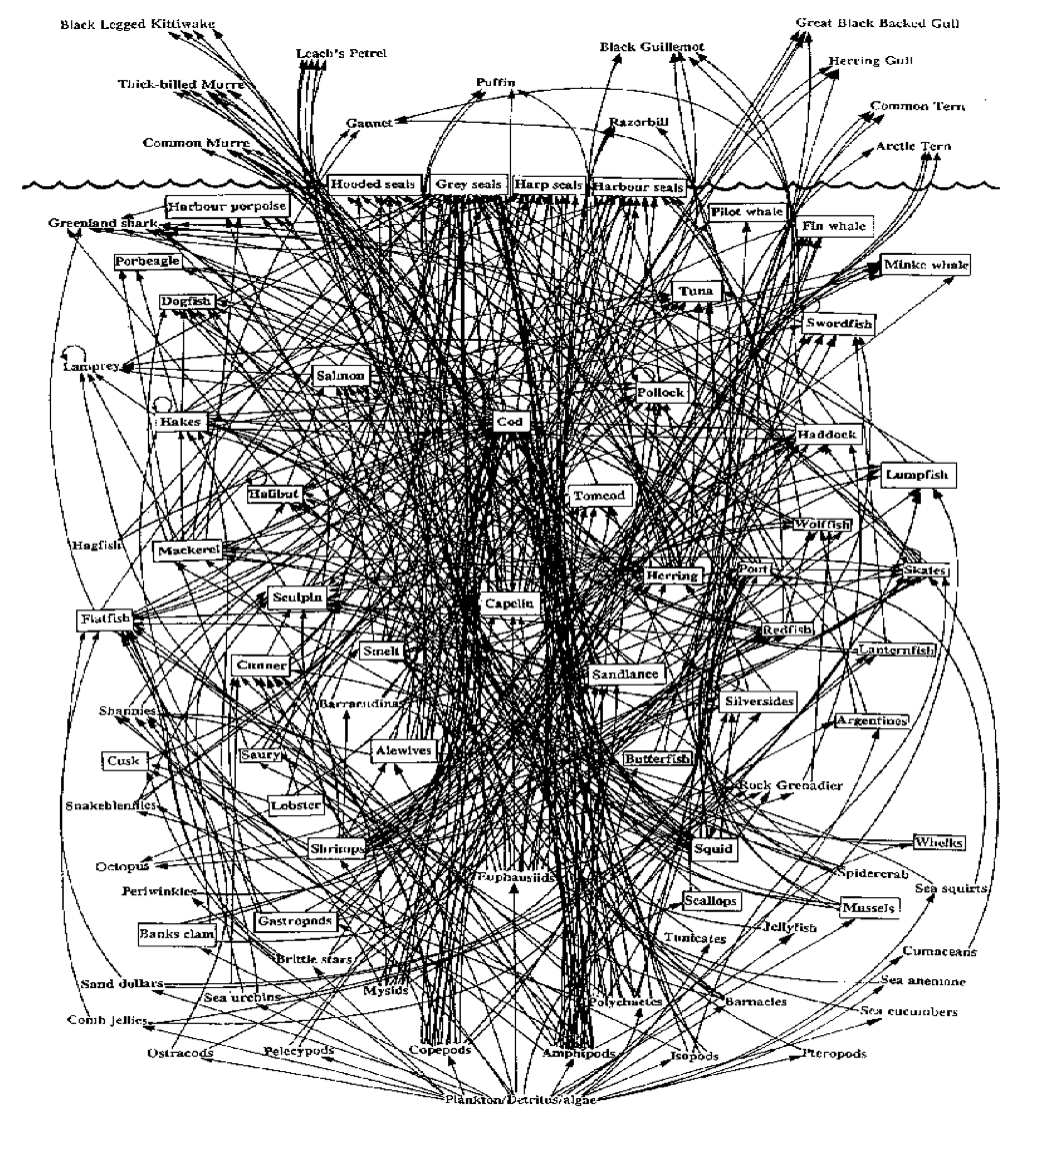
\includegraphics[height=0.85\textheight]{cod_web}
		\end{center}
	
	\end{frame}

%------------------------------

	\begin{frame}
	    
		\begin{center}
			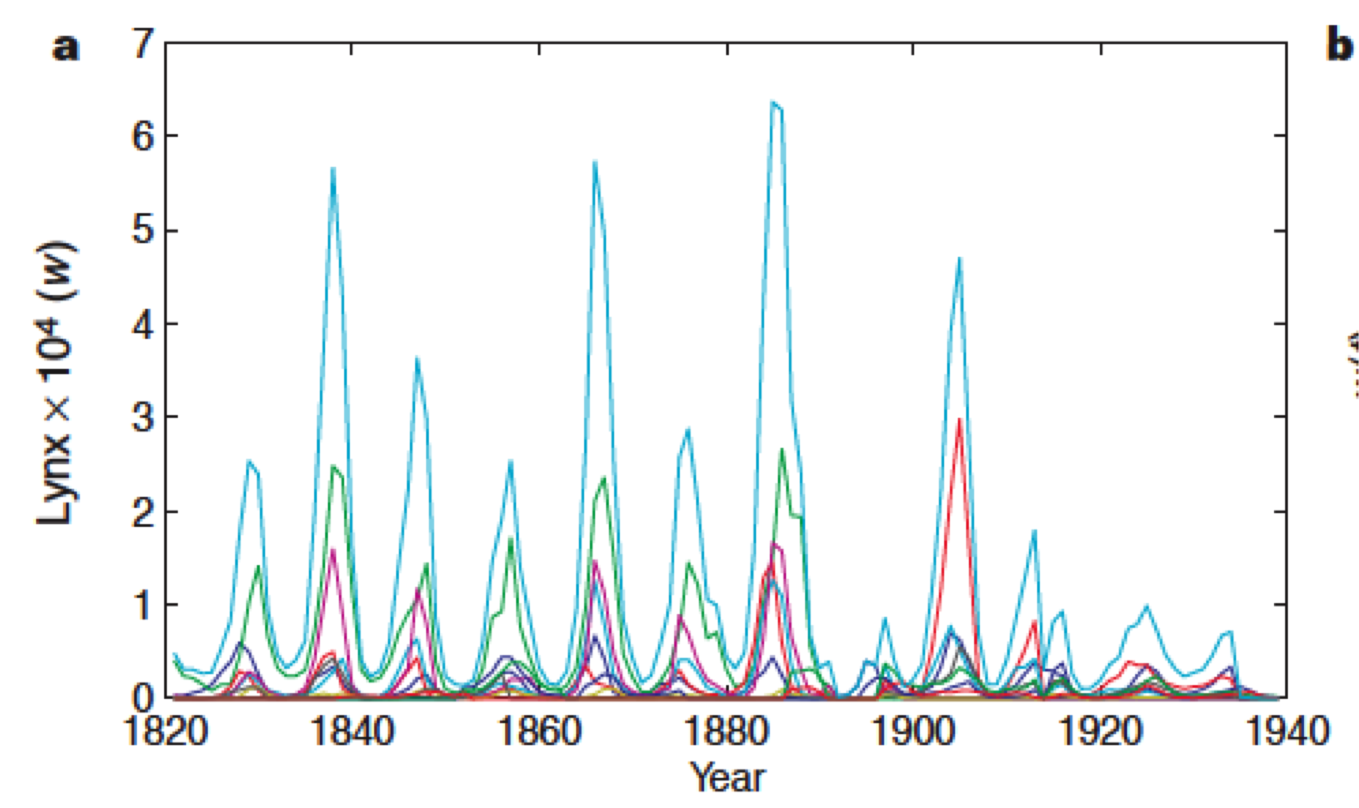
\includegraphics[height=0.75\textheight]{Elton}
		\end{center}
	
	\end{frame}

%------------------------------

	\begin{frame}{Why do we need models?}
	    
Gotelli (1996): \\
\textit{One answer is that we need models because nature is so complex […] The mathematical models act as \textbf{simplified road maps}, giving us some direction and idea of exactly what \textbf{things we should be trying to measure in nature.}}\\	
\vskip 1em

\textit{The models also generate \textbf{testable predictions.}}\\	
\vskip 1em

\textit{The models highlight the \textbf{distinction between the patterns} we see in nature and the different \textbf{mechanisms} that might cause those patterns.}\\	

	\end{frame}

%------------------------------

	\begin{frame}{Some precautionary remarks}
	    
Gotelli (1996):\\
 \textit{The danger is that we build models that are too complex. When this happens, the models may contain many variables that we can never measure in nature.
}\\	
\vskip 1em

\textit{The second danger is that we forget that the models are abstract representations of nature. By carefully focusing on the assumptions of the model, we may be able to pinpoint the places where it departs from reality. 
}\\	

	\end{frame}
%------------------------------

	\begin{frame}{Main types of models}

		\begin{center}
			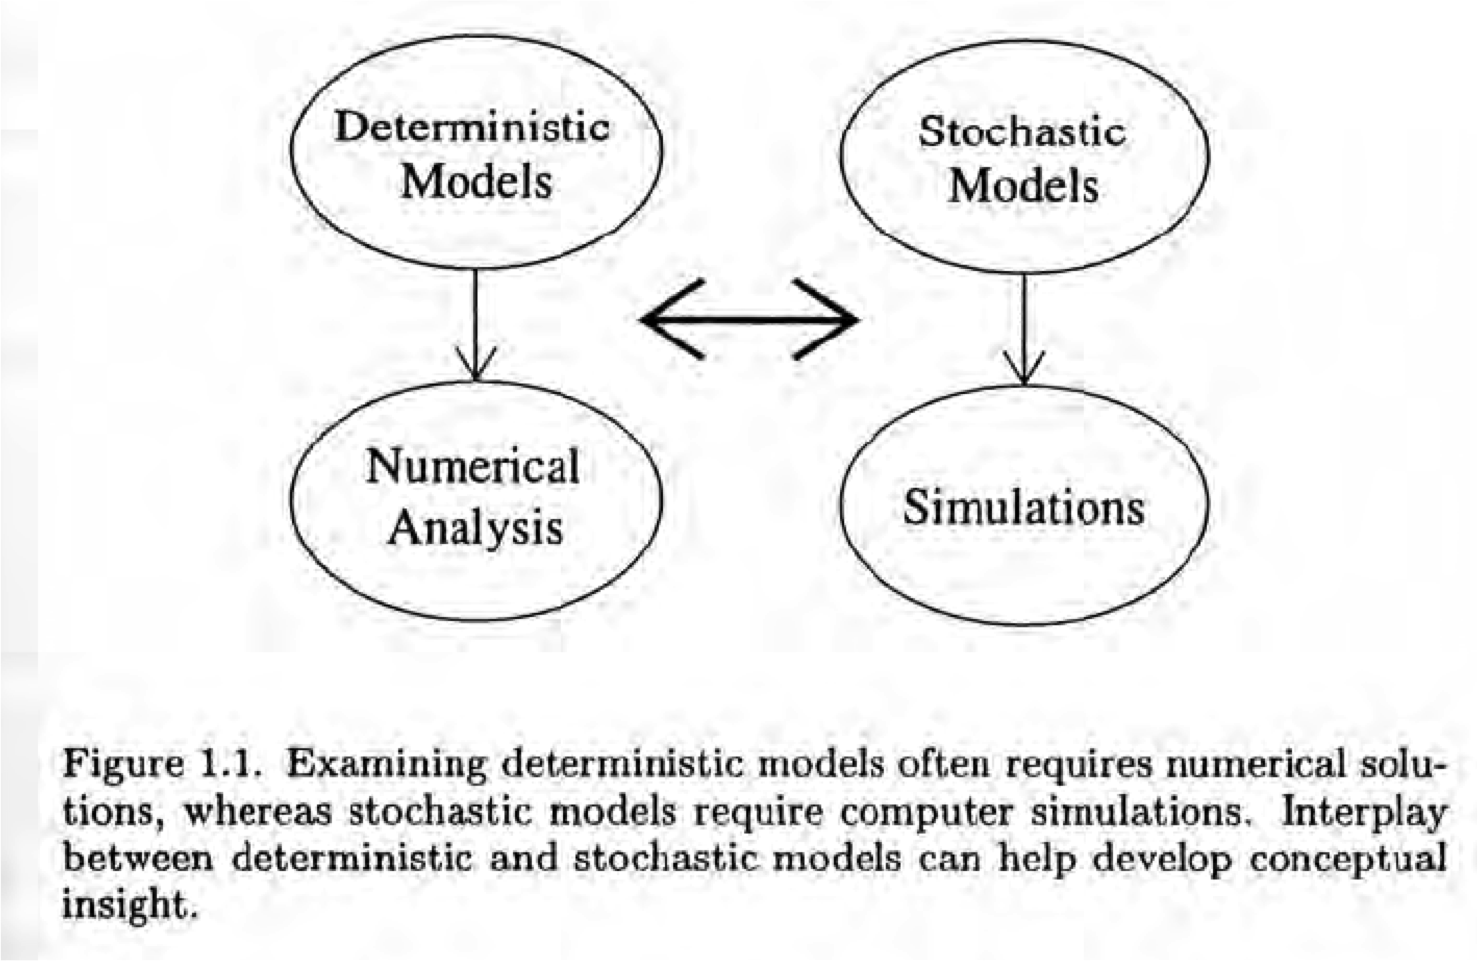
\includegraphics[height=0.75\textheight]{wilson_models}
		\end{center}

	\end{frame}

%------------------------------

	\begin{frame}{Main types of models}{Conceptuals}

		\begin{center}
			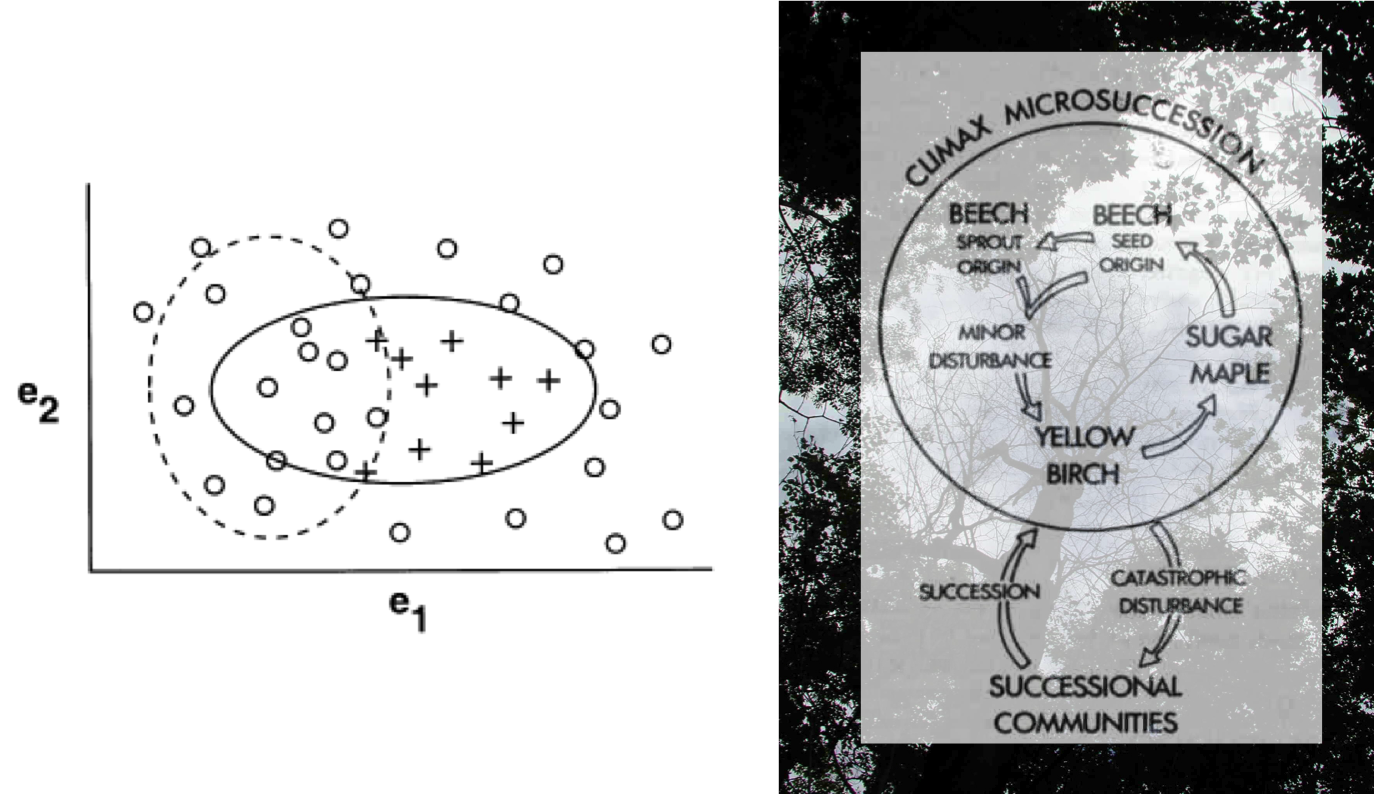
\includegraphics[height=0.65\textheight]{conceptual_model}
		\end{center}

	\end{frame}

%------------------------------

	\begin{frame}{Main types of models}{Statistical}

		\begin{center}
			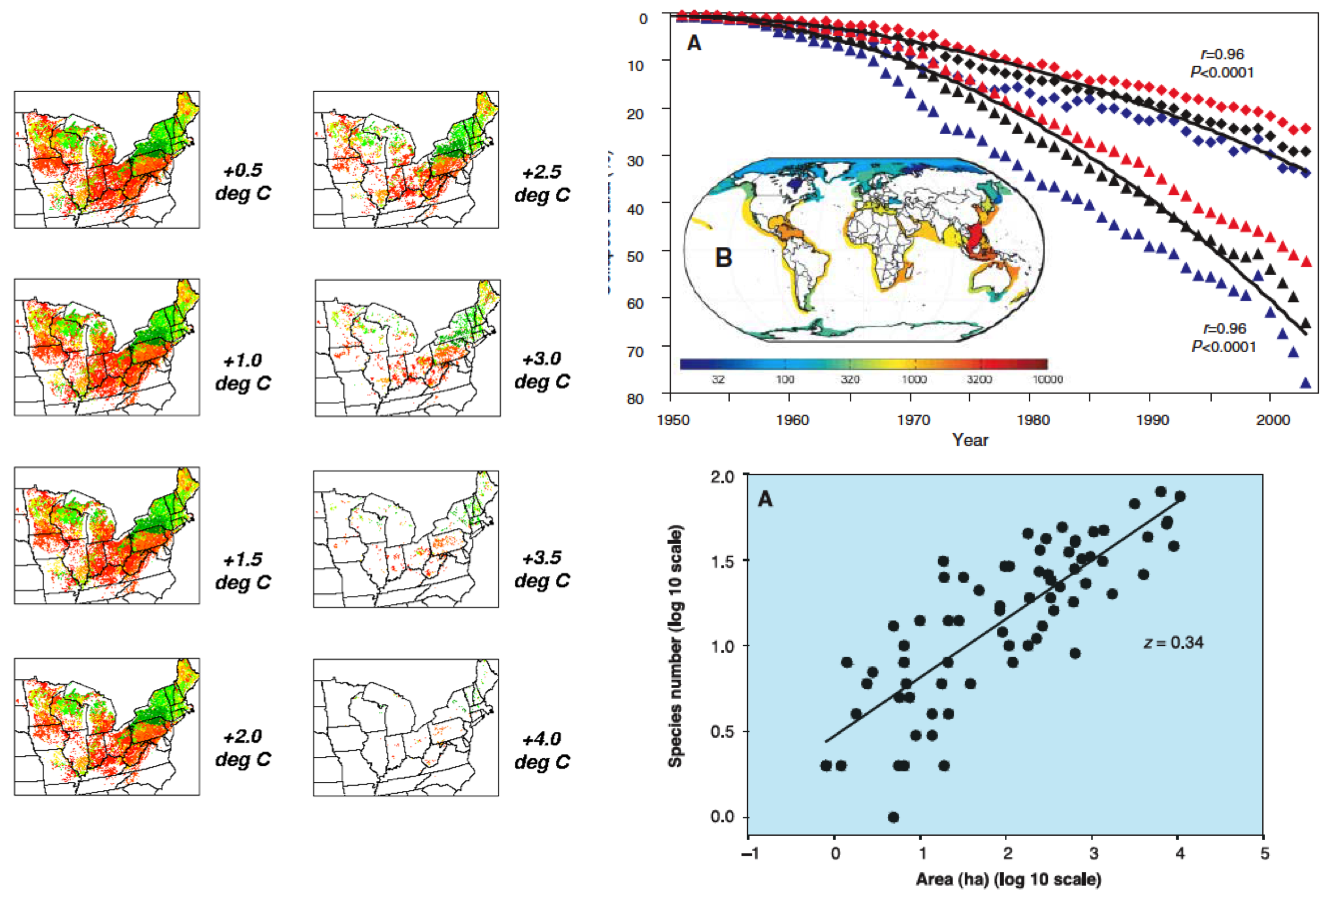
\includegraphics[height=0.75\textheight]{statistical_model}
		\end{center}

	\end{frame}

%------------------------------

	\begin{frame}{Main types of models}{Dynamical}
		\begin{center}
			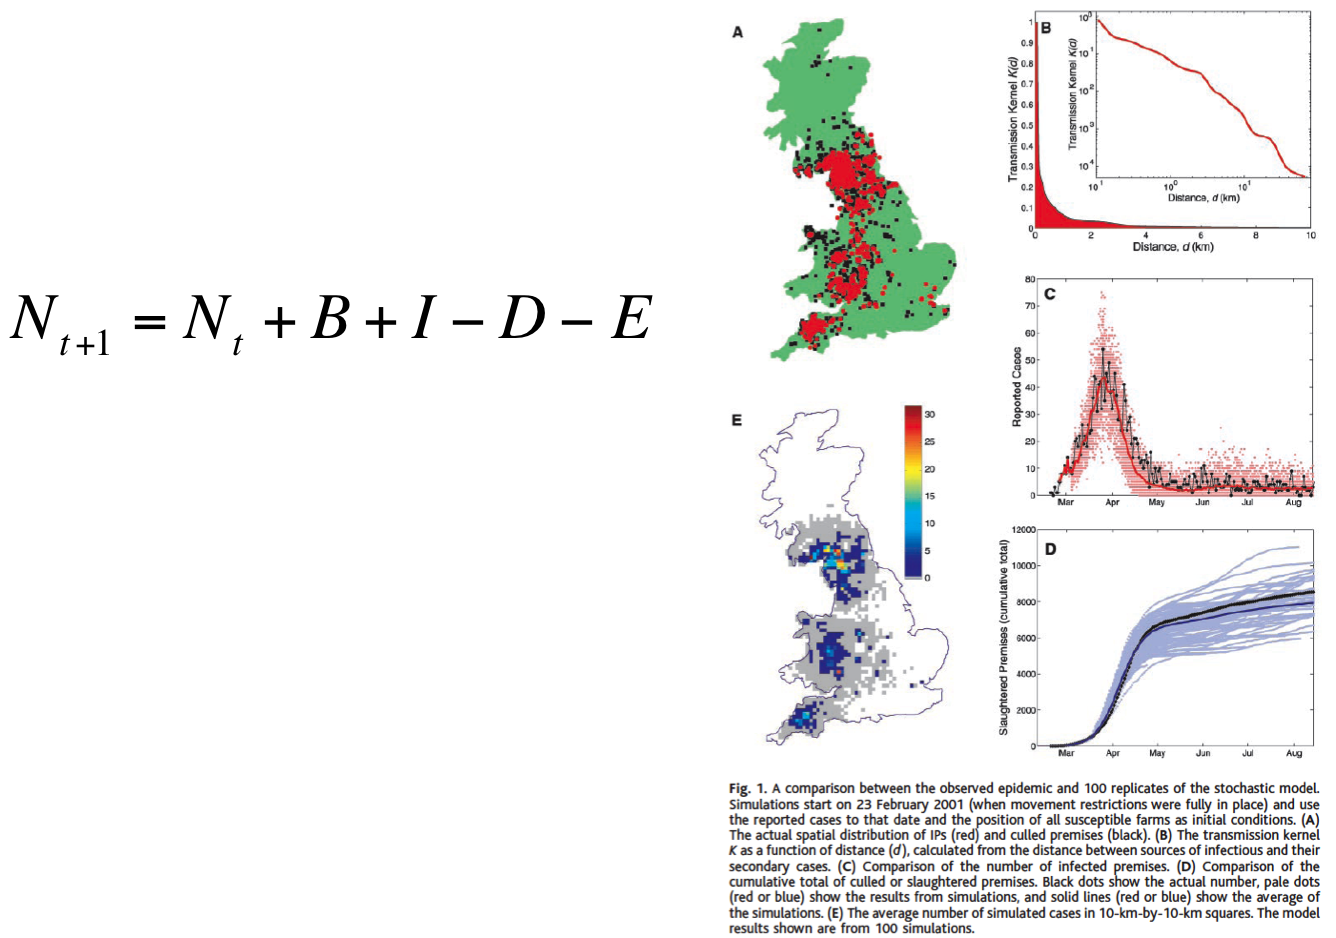
\includegraphics[height=0.75\textheight]{dynamic_model}
		\end{center}
	\end{frame}

%------------------------------

	\begin{frame}{Main types of models}{Deterministic}

		\begin{center}
			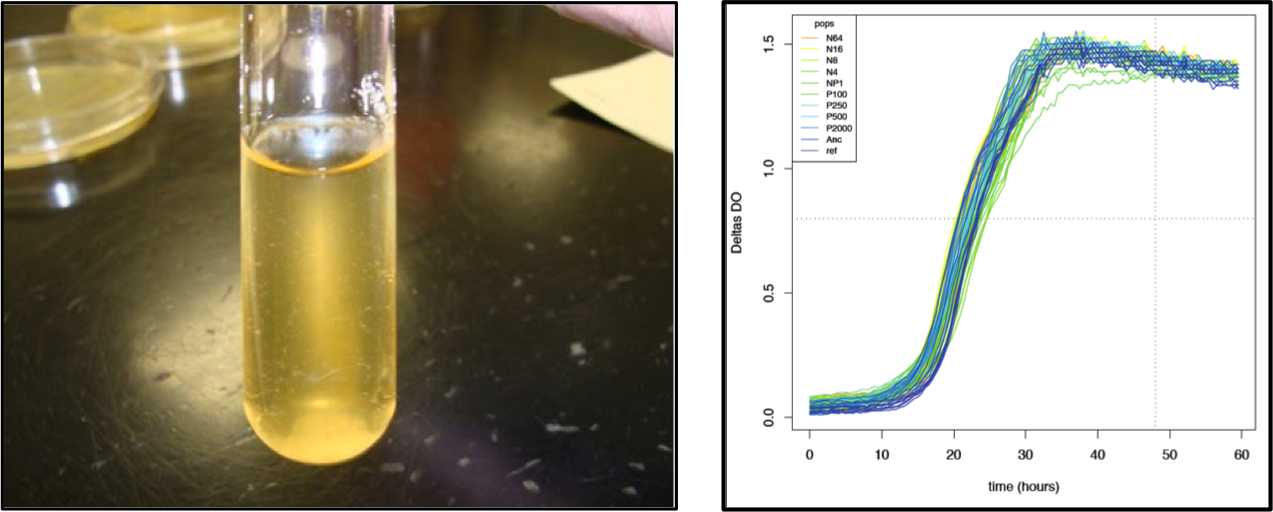
\includegraphics[height=0.5\textheight]{deterministic_model}
		\end{center}

	\end{frame}

%------------------------------

	\begin{frame}{Main types of models}{Stochastic}

		\begin{center}
			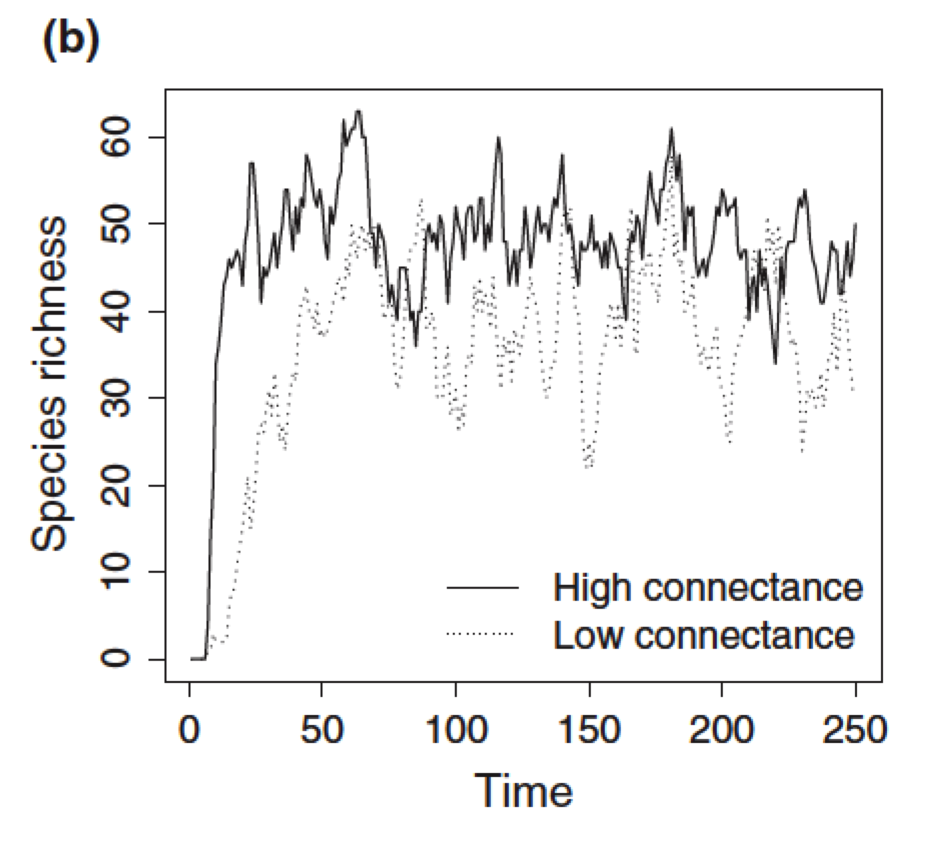
\includegraphics[height=0.75\textheight]{stochastic_model}
		\end{center}

	\end{frame}

%------------------------------

	\begin{frame}{Main types of models}{Cellular automaton}

		\begin{center}
			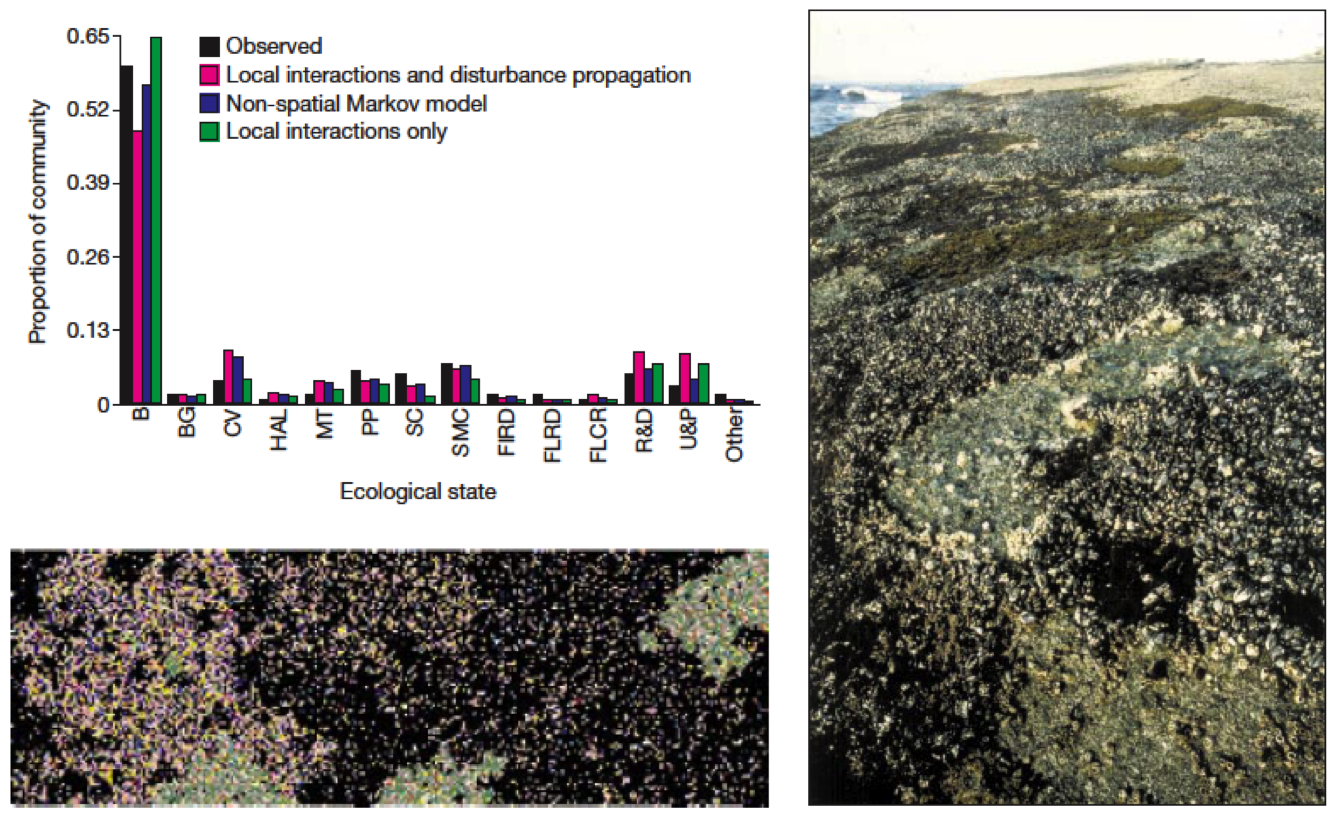
\includegraphics[height=0.65\textheight]{cellular_automaton_model}
		\end{center}

	\end{frame}

%------------------------------

	\begin{frame}{Main types of models}{Individual based models}

		\begin{center}
			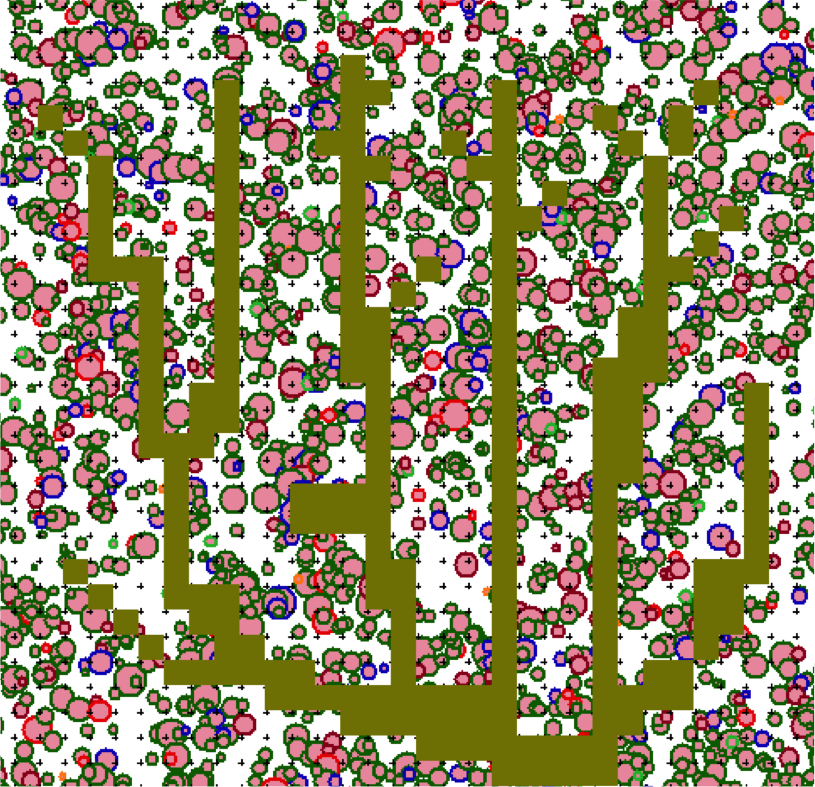
\includegraphics[height=0.65\textheight]{ibm}
		\end{center}

	\end{frame}

%------------------------------

	\section{Objectives}

	\begin{frame}{Conceptual objectives}

	\begin{enumerate}
		\item Distinguish between different types of models
		\item Understand the concept of equilibrium dynamics and its consequences, including mass balance constraints
		\item Understand the R* principle of consumer-resource interactions
	\end{enumerate}

	\end{frame}

%------------------------------

	\begin{frame}{Technical objectives}

	\begin{enumerate}
		\item Formulate ordinary differential equations describing community dynamics of a given ecological system
		\item Analyze the equilibrium states of ordinary differential equations
		\item Perform an invasibility analysis
		\item Compute the Jacobian matrix
		\item Interpret the eigen values of the Jacobian matrix in terms of stability
	\end{enumerate}

	\end{frame}

%------------------------------
%------------------------------

	\section{Definitions}

	\begin{frame}{Ordinary differential equation}{Technical definition}

\textit{An equation containing the derivatives of one or more dependent variables, with respect to one of more independent variables} (Zill - A first Course in Differential Equations)\\	
	\vskip 1em

\textit{A differential equation is a relationship between a function of time \& it's derivatives.} (Braun - Differential equations and their applications)\\	
	\vskip 1em

\textit{Let $f(x)$ define a function of $x$ on an interval $I:a<x<b$. By an ordinary differential equation we mean an equation involving $x$, the function $f(x)$ and one of more of it's derivatives.} (Tenenbaum \& Pollard - Ordinary Differential equations)

	\end{frame}

%------------------------------

	\begin{frame}{Derivative}

\textit{The derivative is a measure of how a function changes as its input changes}\\	
 \vskip 1em

\textit{Loosely speaking, a derivative can be thought of as how much one quantity is changing in response to changes in some other quantity; for example, the derivative of the position of a moving object with respect to time is the object's instantaneous velocity.}

	\end{frame}

%------------------------------
	\begin{frame}{An example with a simple demographic model}

Consider the following model:
$ N_{t+1} = N_t + B + I - D - E$
\vskip 1em

Where:
\begin{itemize}
\item $N$ is population size; \\
\item $B$ is the number of offsprings;\\
\item $I$ is the number of immigrants;\\
\item $D$ is the number of deaths;\\
\item $E$ is the number of emigrants.
\end{itemize}
\vskip 1em

Now, calculate after 3 years the population size of a hare population starting with 10 inidivudals, each giving birth to 5 offsprings per year and with 25\% mortality per winter.

	\end{frame}

%------------------------------

	\begin{frame}{Solution to the geometric growth model}

Consider:\\
$ N_{t+1} = N_t + bN_t + iN_t - dN_t - eN_t = \lambda N_t$
	\vskip 1em

With the intrinsic rate of increase (omitting spatial exchanges):\\
$\lambda = 1 + b - d$ 
	\vskip 1em

For a single time step we obtain:\\
$ N_{t+1} = \lambda N_t$ 
	\vskip 1em

For two time steps:\\
$ N_{t+2} = \lambda N_{t+1} = \lambda (\lambda N_t) = \lambda ^2N_t$  
	\vskip 1em

And for an arbitrary number of time steps:\\
$ N_{t+n} = \lambda ^nN_t$ 

	\end{frame}

%------------------------------

	\begin{frame}{From discrete to continuous time}

	Discrete time:\\
$N_{t+1} = N_t + B - D$\\
$N_{t+1} - N_t = B - D$\\
$\Delta N = B - D$\\
	\vskip 2em

Continuous time: we are interested by the instantenous change in N with a small change in t. \textbf{ Remember the definition of a derivative!}\\
$\frac{dN}{dt} = B - D$

	\end{frame}

%------------------------------
	\begin{frame}{From discrete to continuous time}

The continuous time model (exponential growth):\\
$\frac{dN}{dt} = \beta N - \delta N = rN$ 	
	\vskip 1em

Which has for solution (integrating the differential equation over time):\\
$N(t) = N_0e{rT}$
	\vskip 1em

Given that\\
$ N_{t+n} = \lambda ^nN_t$ 
	\vskip 1em

We obtain the equivalence\\
$\lambda = e^r$
	\vskip 2em

	\end{frame}

%------------------------------

	\begin{frame}{From discrete to continuous time}

		\begin{columns}
			\begin{column}{0.5\textwidth}			
			With $r = \lambda - 1$: WRONG METHOD!
				\begin{center}
					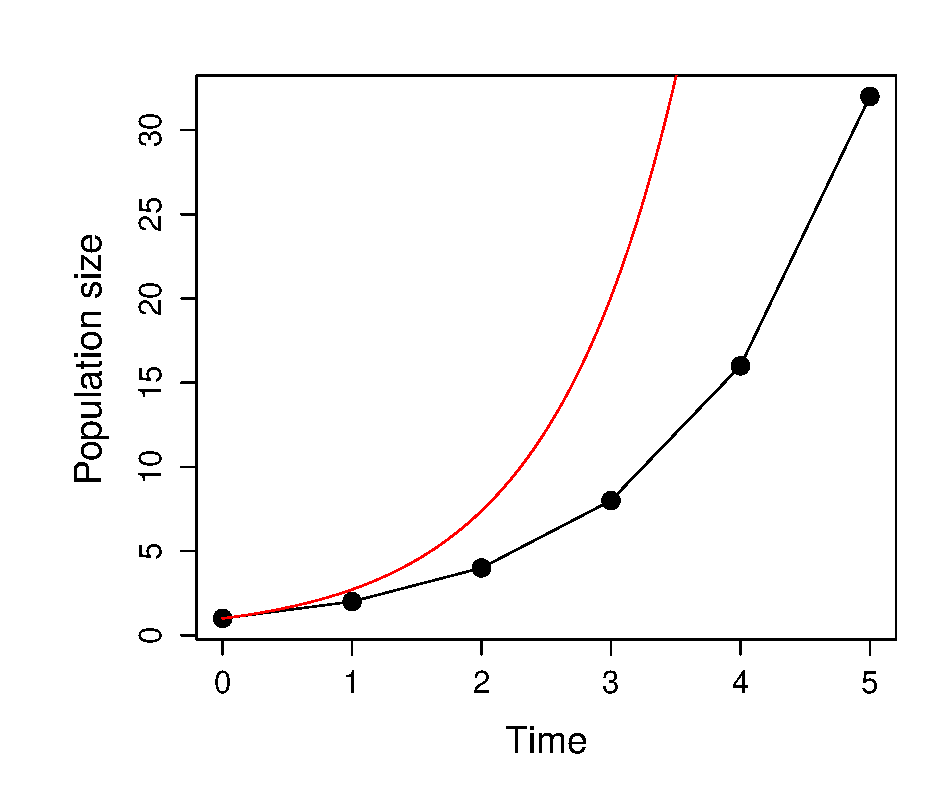
\includegraphics[height=0.5\textheight]{geo_vs_exp_wrong.eps}
				\end{center}
			\end{column}
%----
			\begin{column}{0.5\textwidth}
			The right method:
				\begin{center}
					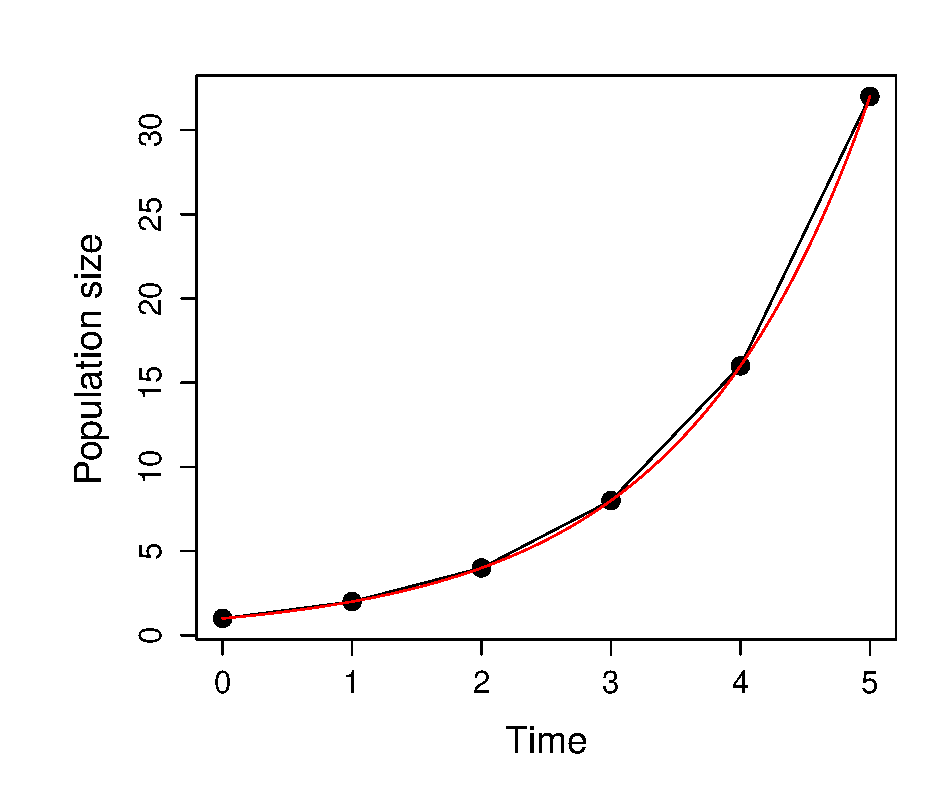
\includegraphics[height=0.5\textheight]{geo_vs_exp_right.eps}
				\end{center}
			\end{column}
		\end{columns}	 

	\alert{Now try to reproduce this figure on R!}

	\end{frame}

%------------------------------

	\section{Steps}

		\begin{columns}
			\begin{column}{0.4\textwidth}			
				\huge{How do we get there?}
			\end{column}
%----
			\begin{column}{0.6\textwidth}
				\begin{center}
					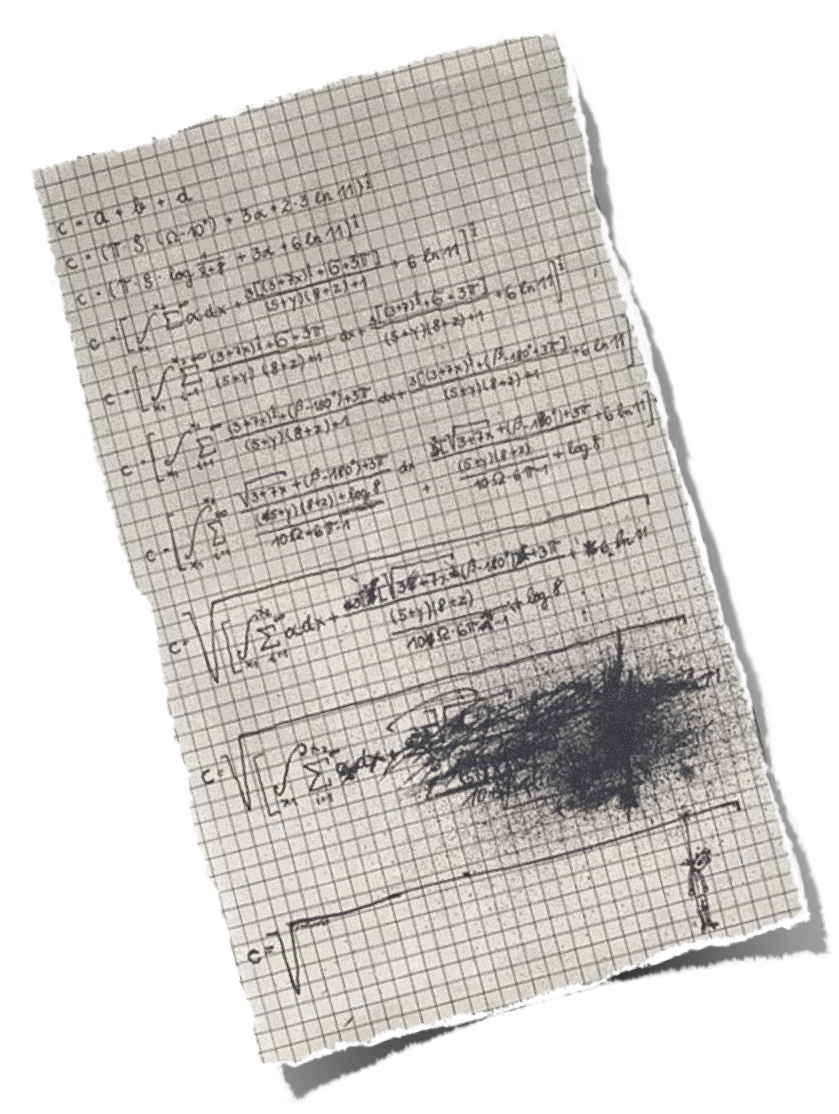
\includegraphics[height=0.9\textheight]{papier.png}
				\end{center}
			\end{column}
		\end{columns}	 

%------------------------------
\begin{frame}{Steps of model analysis}{A standard approach}

	\begin{enumerate}
		\item Conceptualize the system
		\item Formulate the differential equation
		\item Compute equilibrium states
		\item Analyze the different states
		\item Analyze the stability of the equilibrium
	\end{enumerate}

\end{frame}

%------------------------------

	\begin{frame}{Step 1}{Conceptualize the ecosystem}

		\begin{center}
			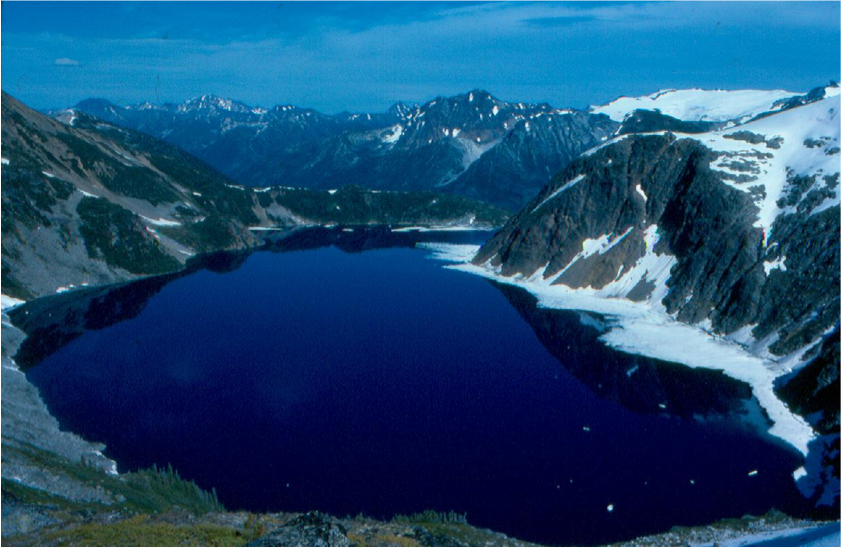
\includegraphics[height=0.5\textheight]{lake.png}
		\end{center}

	\end{frame}
%------------------------------

	\begin{frame}{Step 1}{Conceptualize the ecosystem}

		\begin{center}
			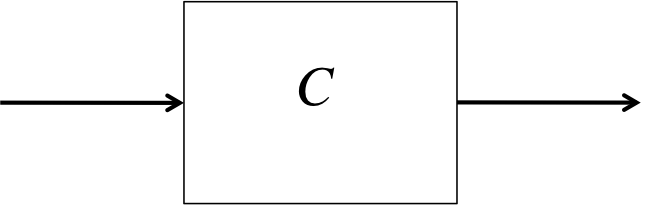
\includegraphics[height=0.4\textheight]{lake_schematic.png}
		\end{center}

	\end{frame}
%------------------------------

	\begin{frame}{Step 2}{Formulate equations}

		\begin{columns}
			\begin{column}{0.65\textwidth}			
				We are looking for an equation describing the instanteneous change in concentration of a 		nutrient. In other words:\\
			$\frac{dC}{dt} = f(t)$
			\vskip 1em

Amount of nutrients coming in: rate of inflow X inflow concentration. In other words: \\
$qC_I$
\vskip 1em

Amount of nutrients going out: rate of outflow X lake concentration. In other words: \\
$qC$
\vskip 1em

Which leads to the instantenous change in concentration:\\
$\frac{dC}{dt} = qC_I - qC$

			\end{column}
%----
			\begin{column}{0.35\textwidth}
				\begin{center}
					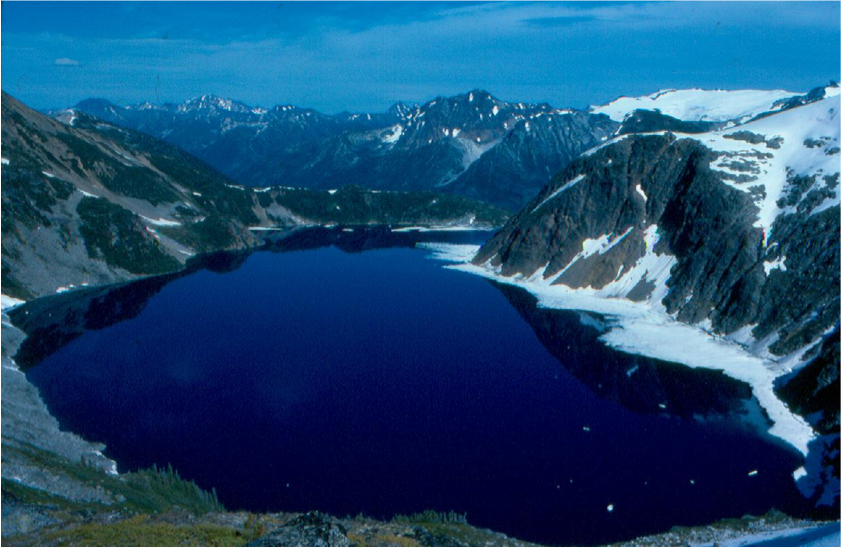
\includegraphics[height=0.2\textheight]{lake.png}
				\end{center}
				\begin{center}
					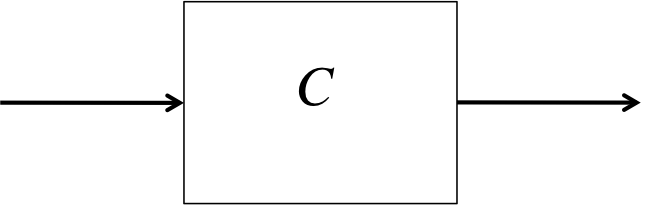
\includegraphics[height=0.15\textheight]{lake_schematic.png}
				\end{center}
			\end{column}
		\end{columns}	 
	\end{frame}

%------------------------------

	\begin{frame}{Step 2}{The law of mass action}

		\textbf{Definition:}\textit{The rate of the reaction is proportional to a power of the concentration of all substances taking part in the reaction}\\
		$ ReactionRate = k[A]^\alpha[B]^\beta$
		\vskip 1em
		
		\textbf{Assumption:} the reaction will only occur if the molecules collide.
		\vskip 1em

		\textbf{Order:} The order of the reaction is the sum of the powers\\
		1st order: $ R1 = k_1[A]$\\
		2nd order: $R2 = k_2[A][B]$

	\end{frame}

%------------------------------

	\begin{frame}{Step 2}{Remember!}

		\begin{itemize}
			\item Conservation of mass and energy
			\item Consistency of units
		\end{itemize}

	\end{frame}
%------------------------------

	\section{Equilibrium}

	\begin{frame}{Step 3}{And now starts the fun part: solving for equilibrium states!}

	The receipe is pretty easy conceptually: set the time derivative to 0 and isolate the variable of interest:\\
$\frac{dC}{dt} = qC_I - qC = 0$
\vskip 1em

Which is equivalent to:\\
$qC_I = qC$
\vskip 1em

And because the $q$ rates cancel each other, we obtain: \\
$\overline{C} = C_I$
\vskip 1em

Where the hat (or often a *) denotes the equilibrium. 

	\end{frame}

%------------------------------

	\begin{frame}{Step 3}{Equilibrium states}

	The method is standard and conceptually simple. Now we need to practice!\\
\vskip 1em

	Consider a tri-trophic food chain obeying the dynamics of the general lotka-volterra equation, where:\\

$ \frac{dN_i}{dt} = N_i(b_i + \sum \alpha_{ij}N_j)$
\vskip 1em

Where the parameter $b_i$ is the intrinsic rate of increase (positive for primary producers, negative for consumers) and the $\alpha_{ij}$ are coefficients giving the per capita effect of species $j$ on species $i$. 

	\end{frame}

%------------------------------

	\begin{frame}{Step 3}{Flipping the problem around}

	The mass-balance assumption: at equilibrium, everything coming in must cancel what goes out. Consequently, we could infer interaction strenght from equilibrium densities. \vskip 1em

Consider the following equilibrium densities for the plant $P$, the herbviore $H$ and the carnivor $C$: \\
$P* = 100$\\
$H* = 10$ \\
$C* = 2$ \vskip 1em

If the intrinsic growth rates are respectively $b_P = 10$, $b_H = -0.3 $, $b_C = -0.1$, what are the interaction coefficients (assuming symmetry of interactions for simplicity)?

	\end{frame}

%------------------------------

	\begin{frame}{Step 3}{Critical conditions for coexistence}

	Not all species need to be present at equilibrium (some densities could equal 0). Therefore we need to assess critical conditions allowing a species to invade a community. Consider a standard plant-nutrient model:\\
$ \frac{dN}{dt} = I - eN - \alpha NP$\\
$ \frac{dP}{dt} = \alpha NP - bP$ \vskip 1em

\begin{enumerate}
	\item Compute the equilibrium nutrient availability in absence of the plant
	\item Compute the plant growth rate when at low density (i.e. P tends to 0)
	\item What is the critical value of $I$ allowing the plant to establish? 
\end{enumerate}

	\end{frame}

%------------------------------

	\begin{frame}{Step 3}{The R* principle}

		\begin{columns}
			\begin{column}{0.5\textwidth}			
				\begin{center}
					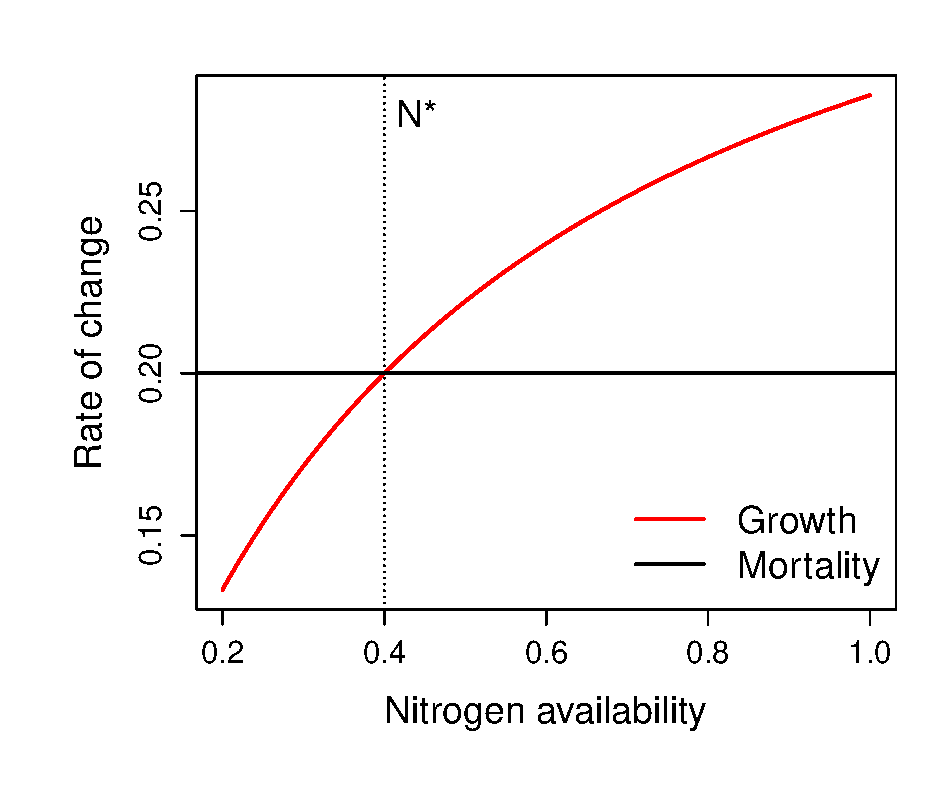
\includegraphics[height=0.5\textheight]{Rstar.eps}
				\end{center}
			\end{column}
%----
			\begin{column}{0.5\textwidth}
				\begin{center}
					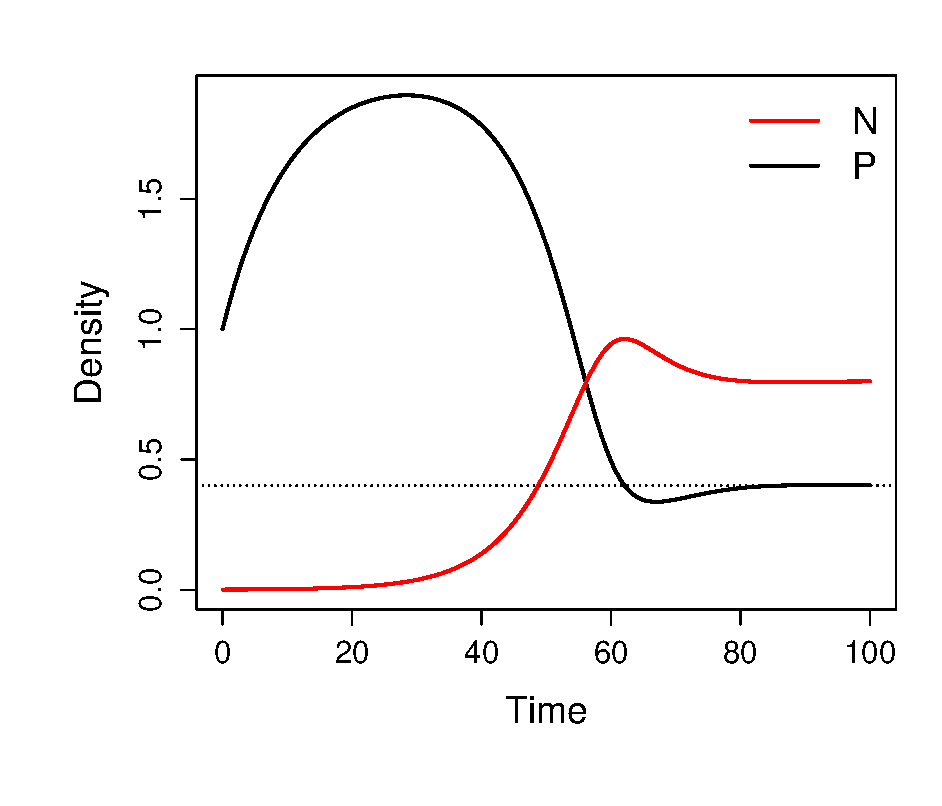
\includegraphics[height=0.5\textheight]{Rstar_dynamics.eps}
				\end{center}
			\end{column}
		\end{columns}
	 
	\textbf{Definition 1:} The R* is the minimal density (or concentration) of resource allowing a species to establish and maintain a population.\\
	\textbf{Definition 2:} The R* is the equilibrium density of the resource in presence of the consumer.
	\end{frame}

%------------------------------
%------------------------------
	\section{Local stability analysis}

	\begin{frame}{Step 4}{Local stability analysis: the big deal!}
	Different types of equilibrium points:
		\begin{center}
			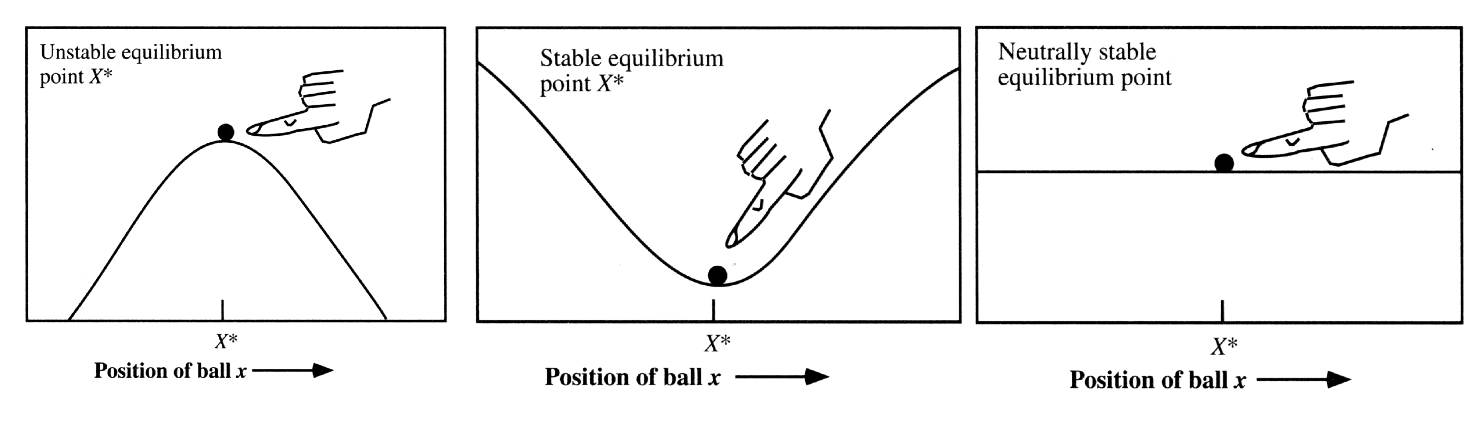
\includegraphics[height=0.3\textheight]{ball.png}
		\end{center}
	\end{frame}

%------------------------------
	\begin{frame}{Step 4}{Local stability analysis: the big deal!}
	Definition of local stability analysis:
		\begin{center}
			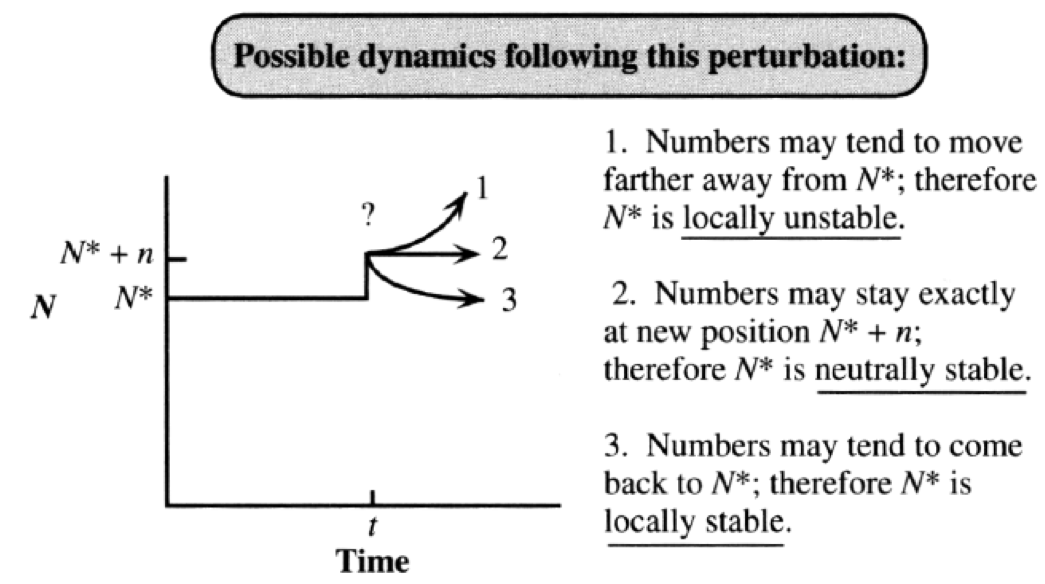
\includegraphics[height=0.5\textheight]{local_stability.png}
		\end{center}
	\end{frame}
%------------------------------
	\begin{frame}{Principle}
	Consider a standard consumer-resource model:\\
	$ \frac{dR}{dt} = R(1-R) - \alpha RC $\\
	$ \frac{dC}{dt} = \alpha RC - mC $
	\vskip 2em

	Which has the following equilibrium:\\
	$R* = m/\alpha$\\
	$C* = \frac{(1-R*)}{\alpha}$\\
	\vskip 2em

	We add small perturbations to this system of equations, defined as:\\
	$ r = R- R*$\\
	$ c = C - C*$\\

	\end{frame}

%------------------------------
	\begin{frame}{Principle (SUITE)}

	We now substitute these quantities in the dynamical equations:\\
	$ \frac{d(R*+r)}{dt} = \frac{dR*}{dt} + \frac{dr}{dt}$\\
	$ \frac{d(C*+c)}{dt} = \frac{dC*}{dt} + \frac{dc}{dt}$\\
	\vskip 1em

	Which by definition reduces to: \\
	$ 0 + \frac{dr}{dt}$\\
	$ 0 + \frac{dc}{dt}$\\
	\vskip 1em

	We are looking for the dynamics of these perturbations in the neighborhood of the equilibrium. In math, it means we are looking to solve the equations:\\
	$ \frac{dr}{dt} = f(r+R*,c+C*)$\\
	$ \frac{dc}{dt} = f(r+R*,c+C*)$\\

	\end{frame}

%------------------------------
	\begin{frame}{Principle (SUITE)}
	Because the functions $f$ and $g$ are often non-linear, there is usualy no solution for the time dynamics $r(t)$ and $c(t)$. There is however a nice and very powerful tool to approximate them. We use a \textit{linearization} around the equilibrum with the Taylor Series. It corresponds to:\\
	$f(x) \cong f(x*) + \frac{f'(x*)(x-x*)}{1!} +\frac{f''(x*)(x-x*)^2}{2!}+...$\\
	\vskip 1em

And for the multivariate situation:
	$f(x,y) \cong f(x*,y*) + \frac{1}{1!}[(x-x*)\frac{\partial f(x*,y*)}{\partial x}+(y-y*)\frac{\partial f(x*,y*)}{\partial y}] +...$\\
	\vskip 1em

Where the symbol $\partial f$ denote partial derivative of function $f$. The partial derivate of $f$ with respect to $x$ is the derivate of $f$ considering only the variable $x$, with other ones fixed as parameters. 

	\end{frame}

%------------------------------

	\begin{frame}{The Taylor approximation}
		\begin{center}
			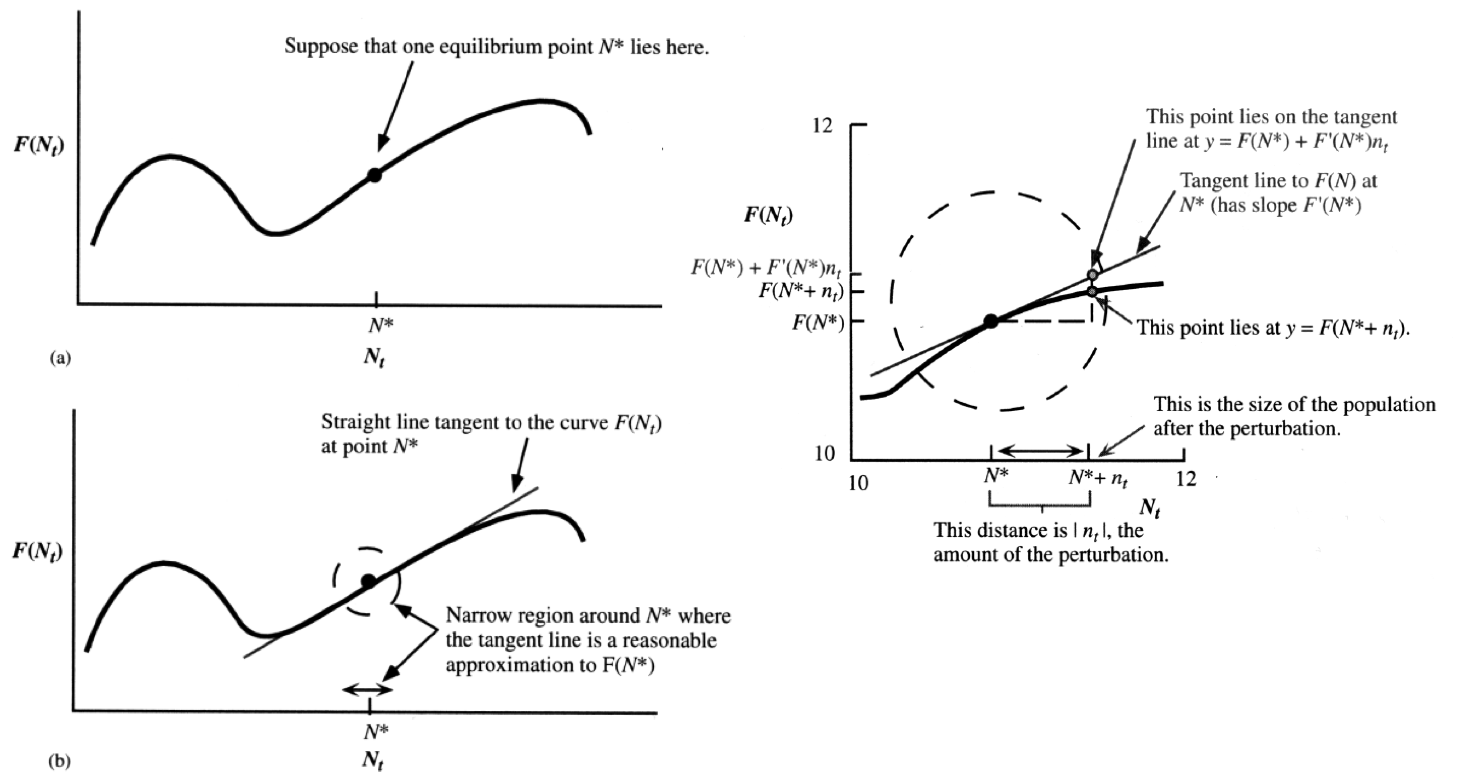
\includegraphics[height=0.7\textheight]{linearization.png}
		\end{center}
	\end{frame}

%------------------------------
	\begin{frame}{Principle (SUITE)}
	The set of partial derivatives gives the following system of equations:\\
	$ \frac{dr}{dt} = r\frac{\partial f(R*,C*)}{\partial R} + c\frac{\partial f(R*,C*)}{\partial C}$\\
	$ \frac{dc}{dt} = r\frac{\partial g(R*,C*)}{\partial R} + c\frac{\partial g(R*,C*)}{\partial C}$\\
	\vskip 1em

	Which written in a matrix format yields:
				\[ J = 
				\begin{bmatrix}
                                	\frac{\partial f(R*,C*)}{\partial R} & \frac{\partial f(R*,C*)}{\partial C} - \\
                                	\frac{\partial g(R*,C*)}{\partial R} & \frac{\partial g(R*,C*)}{\partial C} - \\
				\end{bmatrix} \] 
	\vskip 1em

	Where $\textbf{J}$ is the \textbf{Jacobian matrix}, also referred as the community matrix. The partial derivatives are computed with equilibrum C* and R* values. The Jacobian matrix describes the dynamics of all variables around the equilibrium. The local stability is determined from the Jacobian matrix.

	\end{frame}

%------------------------------
	\begin{frame}[fragile]{Just a trick....}

	Some of you (like me!) might not remember how to derivate complex functions... Here is a trick on R.\\ 

	\begin{lstlisting}	
		# Define the equation to derivate
		dCdt = expression(a*R*C - m*C)

		# Use the function deriv to compute the derivate
		# With respect to C (partial derivate)
		deriv(dCdt,"C")

		# With respect to R
		deriv(dCdt,"R")

		# Evaluate the function
		a = 1
		m = 0.2
		R = 10
		C = 2
		eval(deriv(dCdt,"R"))

		# Be careful with the output!
	\end{lstlisting}

	\end{frame}
%------------------------------
	\begin{frame}{Principle (SUITE)}

	The system dynamics now reads as:\\
	$ \frac{d\textbf{n}}{dt} = \textbf{Jn}$
	\vskip 1em

	Where $\textbf{n}$ is the vector of densities.
	\vskip 1em

	If we remember that the solution to\\
	$\frac{dN}{dt} = rN$\\
	\vskip 1em 

	is:\\
	$N(t) = N_0e^{rT}$\\
	\vskip 1em

	Then we could think there is a solution to this simple system of equations. In order words, the linearization with the Taylor series simplifies the dynamics so that it might be possible to have equations for the dynamics of the small perturbations over time. 

	\end{frame}

%------------------------------
	\begin{frame}{Principle (SUITE)}

	The problem is that in the solution:\\ 
	$N(t) = N_0e^{\textbf{J}T}$
	\vskip 1em

	What does it mean to raise $e$ to the power of matrix $\textbf{J}$? It would be much easier to do it if $\textbf{J}$ would have been a scalar instead of a matrix.	
	\vskip 1em

\end{frame}

%------------------------------
	\begin{frame}{Principle (SUITE)}

	Now the trick is that there is a way to simplify the information contained in a matrix, based on standard linear algebra. It would be much easier if we had a substitution like:\\
	$\textbf{Jn} = \lambda \textbf{n}$
	\vskip 1em

	Where $\lambda$ would be a set of scalars instead of the matrix $\textbf{J}$ . Fortunately, it happens that this equation is exactly the 	definition of eigen values. $\textbf{Jn}$ is the product of a matrix by a vector yielding a vector. 
	\vskip 1em

	\textit{The eigen values are scalars that when multipliying them by the vector $\textbf{n}$, it yields exactly the same result as the matrix multiplication $\textbf{Jn}$}.

	\end{frame}

%------------------------------

	\begin{frame}{Finding eigen values}

	So now we have the situation:\\
	$\textbf{Jn} = \lambda \textbf{n}$\\
	\vskip 1em

	Which after a simple re-arrangement takes the form:\\
	$\textbf{Jn} - \lambda \textbf{n} = 0$\\
	\vskip 1em

	And collecting terms we have:\\
	$(\textbf{J} - \lambda\textbf{I})\textbf{n} = 0$\\
	\vskip 1em
	
	Where $\textbf{I}$ is the identity matrix. This matrix is a square matrix full of 0s, except for the diagonal where all elements are simply 	1. This product yields a matrix full of 0s.

	\end{frame}
%------------------------------

	\begin{frame}{Finding eigen values}

	The values of lambda producing a nonzero solution are given by finding values making the determinant of this matrix equal to 0. In other words, we are looking for the solution of \\
	$det(\textbf{J} - \lambda\textbf{I}) = 0$ 
	\vskip 1em

	The solution to this problem yields the values of $\lambda$s we are looking for. This equation is called the characteristic equation. \\
	\vskip 1em

	\end{frame}

%------------------------------

	\begin{frame}{Finding eigen values}

	As an example (and we'll stay to 2 species for hand calculations!), the determinant of the matrix $\textbf{X}$\\
				\[ X= 
				\begin{bmatrix}
                             	  	a & b \\
                                      c & d 
				\end{bmatrix} \] 
	\vskip 1em

	Is computed as:\\
	$ad-bc$
	\end{frame}

%------------------------------

	\begin{frame}{Finding eigen values}{SUITE}

	We solve the problem using the characteristic equation of the matrix $(\textbf{J} - \lambda\textbf{I})$:\\
	$\lambda^2+B_1\lambda + B_2 = 0$
	\vskip 1em

	Where\\
	$B_1 = -(J_{11}+J_{22})$ 
	and 
	$B_2 = J_{11}J_{22}-J_{12}J_{21}$
	\vskip 1em

	This is a quadratic equation, so we know that it has two roots (ie two eigen values). They are:\\
	$\lambda_1 = \frac{1}{2}(-B_1+\sqrt{B_1^2-4B_2}$ 
	and
	$\lambda_2 = \frac{1}{2}(-B_1-\sqrt{B_1^2-4B_2}$ 
	\vskip 1em

	Ouf, that makes a lot of algebra, but we succeeded!

	\end{frame}

%------------------------------
	\begin{frame}[fragile]{Another trick!}

	Fortunately, there is also a way to compute eigen values numerically. Particularly useful for large matrices. \\
	\begin{lstlisting}
		# Example of computation of eigen values of a very large matrix. 
		# Draw a random matrix for a community of S species
		S = 25
		J = matrix(rnorm(S^2,0,a),nr=S,nc=S)

		# Keep only L links, based on connectance C
		C = 0.3
		rand = matrix(runif(S^2,0,1),nr=S,nc=S) 
		J[rand>C] = 0 

		# Impose competition along the diagonal
		diag(J) = -1

		# Compute eigen values
		res_eigen = eigen(J)$values

		# Keep only the real parts
		real_eigen = as.real(res_eigen)
	\end{lstlisting}

	\end{frame}

%------------------------------
	\begin{frame}{Principle (SUITE)}

	Now coming back to the dynamics of the small perturbations, we have a solution to our system of equations:\\
	$r(t) = k_1e^{\lambda_1t} + k_2e^{\lambda_2t}$\\
	$c(t) = k_3e^{\lambda_1t} + k_4e^{\lambda_2t}$
	\vskip 1em

	Where $\lambda_1$ and $\lambda_2$ are the eigen values of the Jacobian matrix. This system of equation tells us that if all eigen values are negative, then the perturbations will shrink and the system will be stable. Otherwise, they will grow to infinity and the system is unstable.

	\end{frame}

%------------------------------
	\begin{frame}{An example}{Lotka-Volterra predator-prey interactions}

	Consider the classic Lotka-Volterra predator-prey model:
	$\frac{dR}{dt} = bR - aRC = f(R,C)$\\
	$\frac{dC}{dt} = kaRC - dC = g(R,C)$
	\vskip 1em 

	Which has the following equlibrium solution:
	$C* = \frac{b}{a}$\\
	$R* = \frac{d}{ka}$
	\vskip 1em 

	\end{frame}

%------------------------------
	\begin{frame}{An example}{Lotka-Volterra predator-prey interactions}

	The partial derivatives are:\\
	$\frac{\partial f}{\partial R} = b - aC$ and $\frac{\partial f}{\partial C} = - aR$ \\
	$\frac{\partial g}{\partial R} = kaC$ and $\frac{\partial g}{\partial C} = kaR - d$ 
	\vskip 1em

	Which yields the Jacobian matrix:\\
				\[ J= 
				\begin{bmatrix}
                             	  	0 & \frac{-d}{k} \\
                                      kb & 0 
				\end{bmatrix} \] 
	\vskip 1em
	
	And the characteristic equation:\\
	$ \lambda^2+db = 0$

	\end{frame}

%------------------------------
	\begin{frame}{An example}{Lotka-Volterra predator-prey interactions}

	This exemple is a well-known pathologically neutral model. The eigen values are:
	$\lambda = 0 + i\sqrt{bd}$ and $\lambda = 0 - i\sqrt{bd} $
	\vskip 1em

	The dynamics could look like: 

	\end{frame}

%------------------------------
	\begin{frame}{A shortcut for 2 species-systems}{Assessing stability without computing eigen values}
	
	This technique is pretty heavy, but in some cases it might be simpler using an alternative approach (known as the Routh-Hurvitz criteria) but nonetheless based on the same principle. Remembering the above solution for eigen values\\
	$\lambda_1 = \frac{1}{2}(-B_1+\sqrt{B_1^2-4B_2}$ \\
	and \\
	$\lambda_2 = \frac{1}{2}(-B_1-\sqrt{B_1^2-4B_2}$ 
	\vskip 1em

	The conditions for a stable system to occur are that $B_1>0$ and $sqrt{B_1^2-4B_2}<B_1$. Re-arranging the last condition yields that:
	$B_1 = -(J_{11}+J_{22}) > 0 $\\
	and \\
	$B_2 = J_{11}J_{22}-J_{12}J_{21} > 0 $
	\vskip 1em
	
	These conditions could then be rapidly assessed using only the sign structure of the matrix. 

	\end{frame}

%------------------------------

	\begin{frame}{Summary of the receipe}
	\begin{enumerate}
		\item Compute the equilibrium
		\item Calculate partial derivatives
		\item Build the Jacobian matrix
		\item Calculate the eigen values
			\begin{itemize}
				\item $\lambda < 0$: stable
				\item $\lambda > 0$: unstable
				\item $\lambda = 0$: neutrally stable
				\item No imaginary part: smooth return
				\item Imaginary part: oscillations 
			\end{itemize}
		\end{enumerate}
	\end{frame}

%------------------------------

	\begin{frame}{Exercises}
		
		Consider the famous M\&W model of island biogeography:
		\begin{center}
			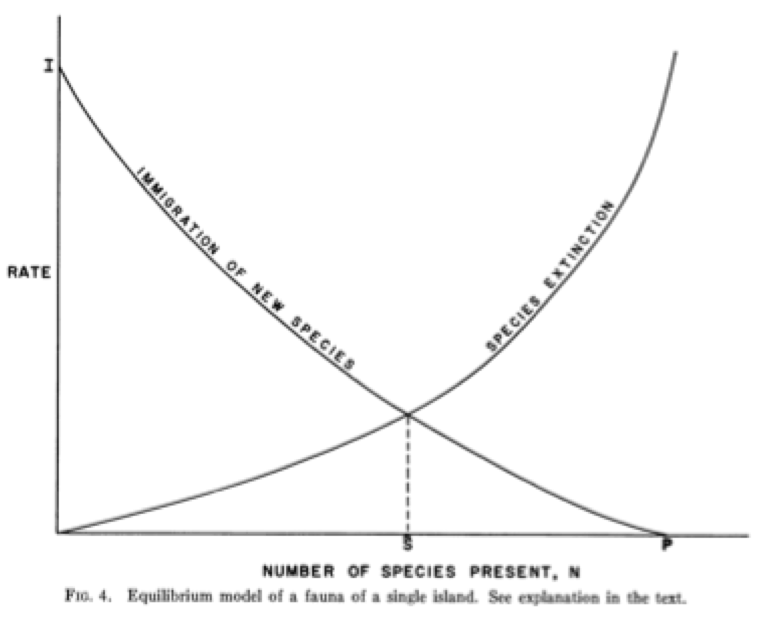
\includegraphics[height=0.4\textheight]{IBT.png}
		\end{center}
		
		\begin{itemize}
			\item Formulate the equation describing the dynamics of species richness on islands
			\item Now consider that $e = \frac{epsilon}{A^b}$ and solve the model at equilibrium
			\item What is the rate of change of equilibrium species richness with habitat destruction? Is 10\% habitat destruction affecting more small or large islands?
			\item Calculate the stability of equilibrium species richness
		\end{itemize}

	\end{frame}

%------------------------------

	\begin{frame}{Exercises}
		
		Consider another classic model: Lotka-Volterra equations for competition.
		$ \frac{dN_i}{dt} = rN_i(1-\frac{\alpha_{ij}N_j}{K_i} -\frac{N_i}{K_i} )$
		\vskip 1em

		\begin{center}
			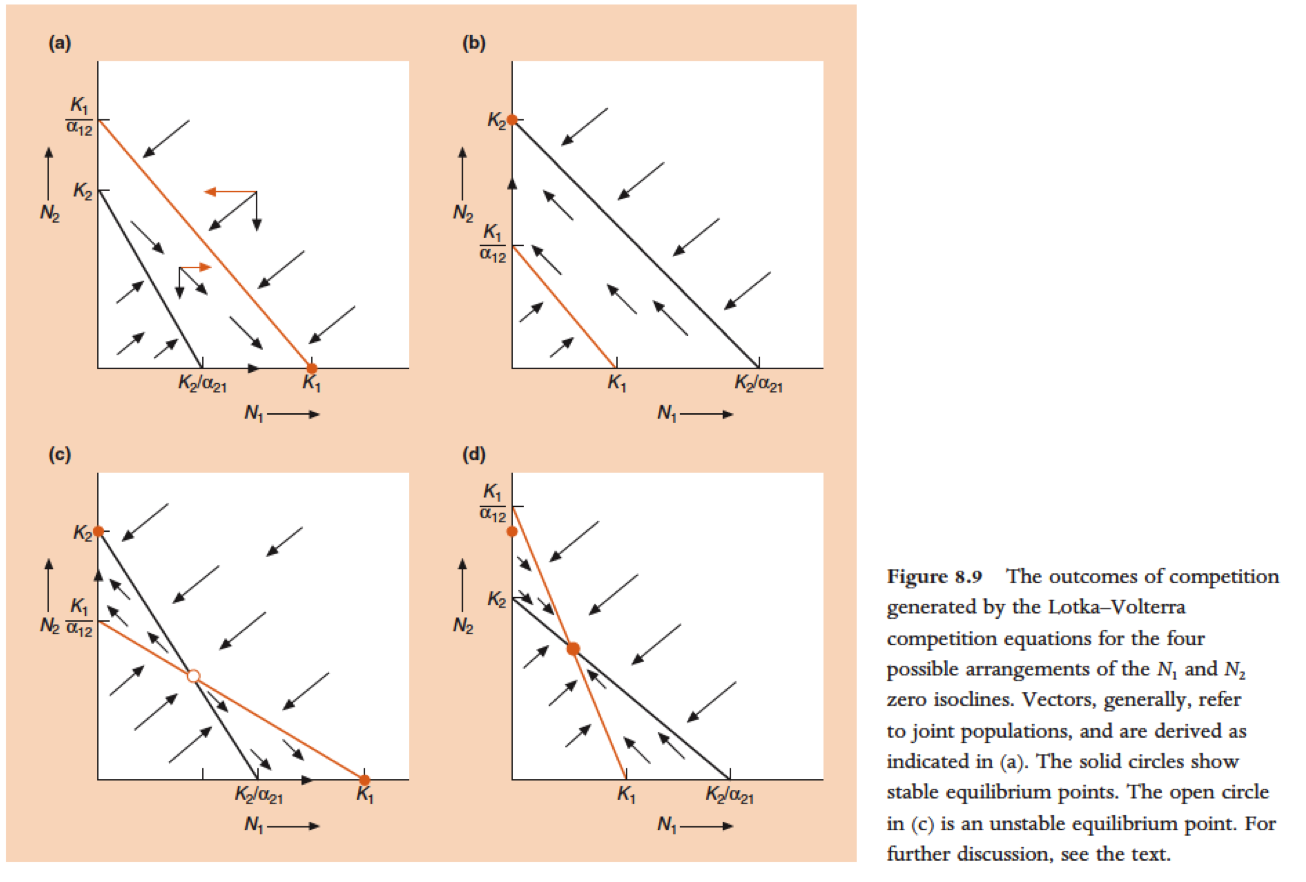
\includegraphics[height=0.4\textheight]{lv_compet.png}
		\end{center}
		
		\begin{itemize}
			\item Solve the model at equilibrium with two species
			\item Compute the stability of the model with one of the two species absent. What happens if $K_1 = K_2 = 1$ and $\alpha_{ij} = \alpha_{ji} = 0.5$?
		\end{itemize}

	\end{frame}

%------------------------------

	\begin{frame}{Exercises}
		
		Consider another classic model: Lotka-Volterra equations for competition.

		\begin{center}
			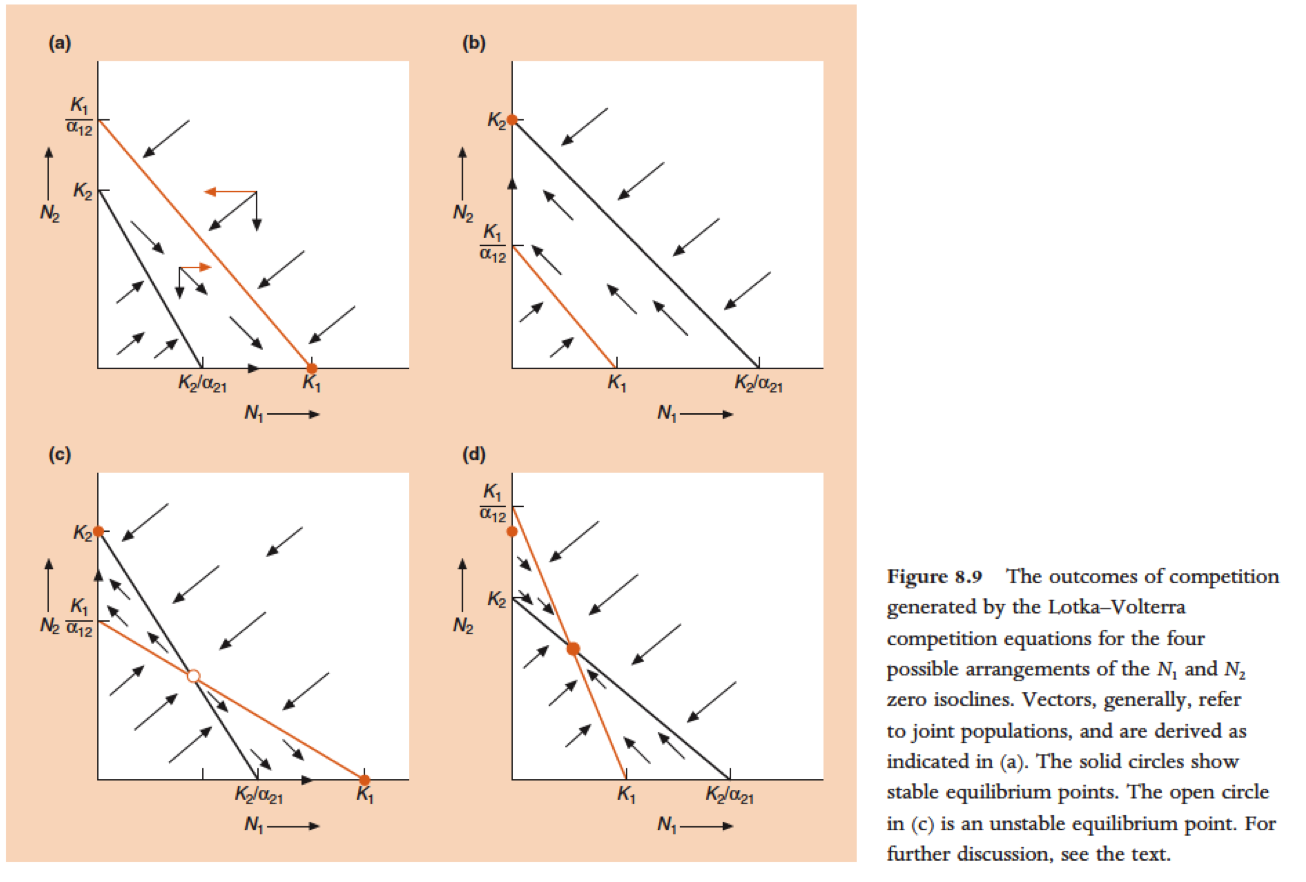
\includegraphics[height=0.5\textheight]{lv_compet.png}
		\end{center}
		
		$ \frac{dN_i}{dt} = rN_i(1-\frac{\alpha_{ij}N_j}{K_i} -\frac{N_i}{K_i} )$

		\begin{itemize}
			\item Solve the model at equilibrium with two species
			\item Compute the stability of the model with one of the two species absent. What happens if $K_1 = K_2 = 1$ and $\alpha_{ij} = \alpha_{ji} = 0.5$?
		\end{itemize}

	\end{frame}

%------------------------------
%------------------------------
\end{document}